\documentclass[final,hyperref={pdfpagelabels=false}]{beamer}

\usepackage[orientation=portrait,size=a0,scale=0.79]{beamerposter}

\usetheme{HorGagSawPos} % beamerthemeHorGagSawPos
\usepackage[english]{babel} % English language/hyphenation

\usepackage{amsmath,amsthm,amssymb,latexsym} % For including math equations, theorems, symbols, etc

\usepackage{multirow} % multirow in tables
\usepackage{hhline} 

% to work with tabular
\usepackage{xcolor,colortbl}

% align in arrays
\usepackage{array}
\newcolumntype{L}[1]{>{\raggedright\let\newline\\\arraybackslash\hspace{0pt}}m{#1}}
\newcolumntype{C}[1]{>{\centering\let\newline\\\arraybackslash\hspace{0pt}}m{#1}}
\newcolumntype{R}[1]{>{\raggedleft\let\newline\\\arraybackslash\hspace{0pt}}m{#1}}

%\usepackage{times}\usefonttheme{professionalfonts}  % Uncomment to use Times as the main font
%\usefonttheme[onlymath]{serif} % Uncomment to use a Serif font within math environments

%\boldmath % Use bold for everything within the math environment

\usepackage{booktabs} % Top and bottom rules for tables

\graphicspath{{figures/}} % Location of the graphics files

\usecaptiontemplate{\small\structure{\insertcaptionname~\insertcaptionnumber: }\insertcaption} % A fix for figure numbering

%----------------------------------------------------------------------------------------
%	TITLE SECTION 
%----------------------------------------------------------------------------------------

\title{\huge Towards the HPC-inference of causality networks\\[0.8ex] from multiscale economical data} % Poster title

\author{\hfill\Large Illia~Horenko$^{ 1}$, Patrick~Gagliardini$^{ 1}$, William~Sawyer$^{ 2}$, Luk\'{a}\v{s} Posp\'{i}\v{s}il$^{ 1}$}

\institute{\large \hfill  $^{1}$ Universit\`a della Svizzera Italiana (USI Lugano),
				  $^{2}$ Swiss National Supercomputing Centre (CSCS/ETH Zurich),\\[1ex]
			\hfill {\tt \large [illia.horenko@usi.ch, patrick.gagliardini@usi.ch, william.sawyer@cscs.ch, lukas.pospisil@usi.ch]} }

%----------------------------------------------------------------------------------------

\begin{document}

\addtobeamertemplate{block end}{}{\vspace*{2ex}} % White space under blocks

\begin{frame}[t] % The whole poster is enclosed in one beamer frame


\begin{columns}[t] % The whole poster consists of two major columns, each of which can be subdivided further with another \begin{columns} block - the [t] argument aligns each column's content to the top

\begin{column}{.01\textwidth}\end{column} % Empty spacer column

\begin{column}{.48\textwidth} % The first column

%----------------------------------------------------------------------------------------
%	Focus of the project
%----------------------------------------------------------------------------------------

\begin{block}{Focus of the project}

Analysis of large amounts of economical data and data-driven inference of causality relations between different
components of economical systems  is one of the central problems in modern computational finance and economics. 
The task of proper mathematical description and adequate causality understanding for the economical data is hampered
by the multiscale nature of the underlying processes, resulting from the presence of different temporal and spatial, i.e. regional, sectorial and global, scales.

\vskip2ex

\noindent Important challenges are: 
\begin{itemize}
 \item[(i)] an investigation of the mutual causality influences of different economic observables and their spatial (e.g., regional) and temporal (e.g., associated with the business cycle) evolution, 
 \item[(ii)] identification of the most important exogenous impact factors that play a role in their dynamics, 
 \item[(iii)] proper mathematical and statistical description of the influences coming from the unresolved/latent scales and factors. 
\end{itemize}
The solution of these problems can be enhanced by  analysis of  a causality network inferred from the data.  This network is a directed weighted graph with edges representing the causality relations between the  different economical variables, exogenous factors, etc. (situated at the vertices of this causality graph). Analysis of this graph would allow to understand the most important features of the underlying complex economical system.

\vskip2ex

{\color{blue}
\noindent Milestone questions about the targeted economical data:
\begin{enumerate}
  \item {\color{blue}Is there a causality relation between different sectors of the economy with respect to the credit risk migrations?'}
  \item {\color{blue}What is the most effective implementation of the multiscale causality inference framework in the embarassingly-parallel case?}
  \item {\color{blue}Are there any statistically-significant causality impacts from other sectors on the companies inside of the `Banking and Finance' sector?}
  \item {\color{blue}Among all of the considered alternatives and platforms, what is the most scalable implementation for multiscale causality inference?}
\end{enumerate}
}
%\vskip2ex
\end{block}

%----------------------------------------------------------------------------------------
%	Understanding Causality
%----------------------------------------------------------------------------------------
            
\begin{block}{Understanding Causality}

In its purest deterministic sense, there is a causal relationship between events if one implies that another has occurred.  
In reality, such causal relationships can generally only be determined from first principles on a small spatial/temporal scale, with little data involvement. 
For larger scales and/or larger data involvement, mathematical or statistical models are required from whence causality can be inferred.

\begin{columns}[T]
\begin{column}{0.05\linewidth}\end{column}
\begin{column}{0.9\linewidth}
	\begin{figure}[H]
		\begin{center}
			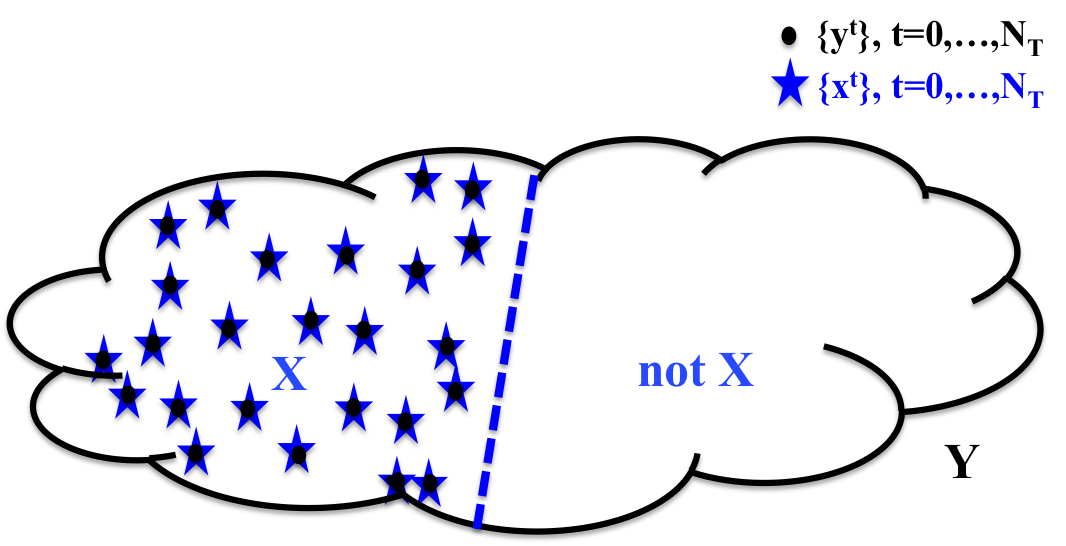
\includegraphics[width=0.5\linewidth, angle=0, clip = true]{figures/Deterministic_Causality.png}
			\hfil
			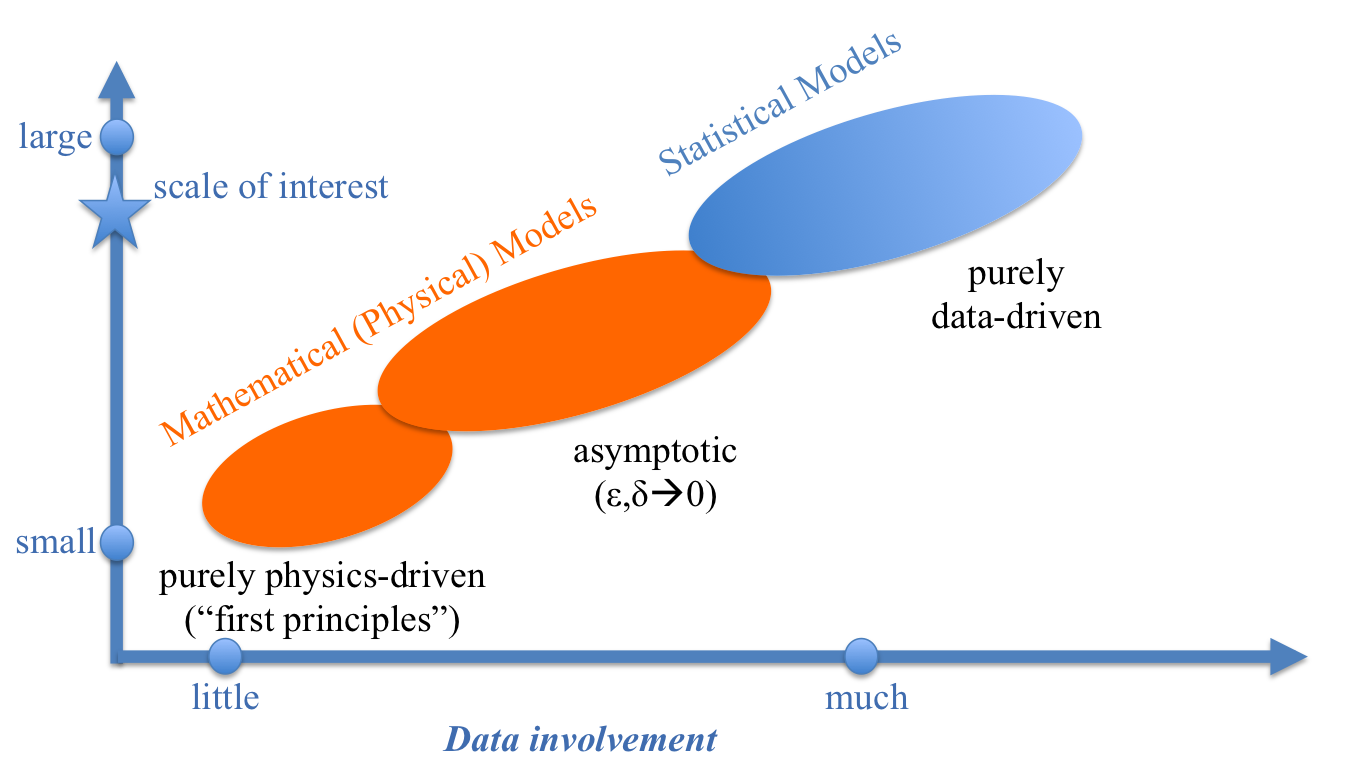
\includegraphics[width=0.5\linewidth, angle=0, clip = true]{figures/Causality_Model_or_Data_Driven.png}
			\caption{Deterministic Causality (left):  $X$ has a causality impact on $Y$ if for any $t$, event $y^t$ is happening if and only if event $x^t$ happened.  In real applications a data model is required, but the realm of applicability (right) determines whether the causality inference is driven by the model or by the data .}
		\end{center}
	\end{figure}
\end{column}	
\begin{column}{0.05\linewidth}\end{column}
\end{columns}

\vskip2ex

\underline{\large Granger Causality:} 
The standard causality inference measures the ability of predicting the future values of a time series (e.g., $y^{t+\tau}$) using past values of another time series (e.g., $x^t,x^{t-\tau},\dots,x^{t-q\tau}$), where $\tau$ is a time step and $q\tau$ is a maximal time lag \cite{granger69}.  The predictive models that have been deployed first to measure such a causality relation between $y$ and $x$ were linear {\bf A}uto{\bf R}egressive models with e{\bf X}ternal impact factors (ARX-models) \cite{brockwell2002}:
\begin{eqnarray}
\label{eq:ARX}
y^{t+\tau}&=&\mu+\sum_{i=0}^p A_iy^{t-i\tau}+\sum_{j=0}^q B_jx^{t-j\tau}+\sigma\left(t\right),
\end{eqnarray}
where $\{\mu,A_0, A_1,\dots,A_p,B_0, B_1,\dots,B_q\}$ are the ARX-model parameters that can be estimated from the available time series for $x$ and $y$ (e.g., deploying the maximum likelihood method) and $\sigma\left(t\right)$ is some stochastic noise process \cite{brockwell2002}. Then, the variable $x$ has a Granger causality relation to the variable $y$ if and only if at least one of the $B_j$ is statistically-significantly different from zero.

\vskip2ex

\underline{\large Limitations:}
Granger causality may lead to biased results.  This bias might be amplified and lead to a completely wrong inference of the causality relations from the data, if the underlying model assumptions of standard causality inference methods (e.g., like the intrinsic linearity of the Granger causality measures) are not fulfilled.

%\vskip2ex
\end{block}


%----------------------------------------------------------------------------------------
%	Probabilistic (Bayesian) Causality
%----------------------------------------------------------------------------------------

%\begin{block}{Probabilistic (Bayesian) Causality}

%In contrast to typical applications from computational sociology (where the underlying network/graph is mostly available explicitly, e.g., in the form of a social network directly describing the observed connections and relations between the individuals), in a context of economical data these causality network structures are often implicit, difficult to measure, and need to be inferred from the very large sets of available data.  The law of total probability can assist us:

%\vskip2ex

%\underline{\large Law of Total Probability:} 
%If $B_1, B_2, B_3,\cdots$ is a partition of the sample space $S$, then for any event $A$ we have
%\begin{displaymath}
%P(A)=\sum_{i} P(A \cap B_i)=\sum_{i} P(A | B_i) P(B_i).
%\end{displaymath}

%\vskip2ex

%\noindent In this project we investigate the case that both $X$ and $Y$ are driven by an (unobserved) process $U$ with different lags, e.g., 
%unresolved scale impacts. We start by defining the probability vectors 
% TODO: $\Lambda(t)=(\bP\left[y^t|x_1^t \text{ and } u^t \right],\dots,\bP\left[y^t|x_n^t \text{ and } u^t\right],$ $ \bP[y^t \text{  and not one of } x_i^t])$,  $P_x^t=\left(\bP\left[x_1^t \text{ and } u^t \right],\dots,\bP\left[x_n^t \text{ and } u^t \right],1\right)$ and a variable $P^t_y=\bP\left[y^t \right] $. 
%Then the probability of observing $y^t$ together with $x_1^t,\dots,x_n^t$ and $u^t$ can be written as a scalar product of these two vectors:

%\begin{equation}
%\label{eq:full_prob}
%P_y^t = \Lambda^{\dagger}(t)P^t_x,
%\end{equation}

%\begin{columns}[T]
%\begin{column}{0.05\linewidth}\end{column}
%\begin{column}{0.9\linewidth}
%	\begin{figure}[H]
%		\begin{center}
%			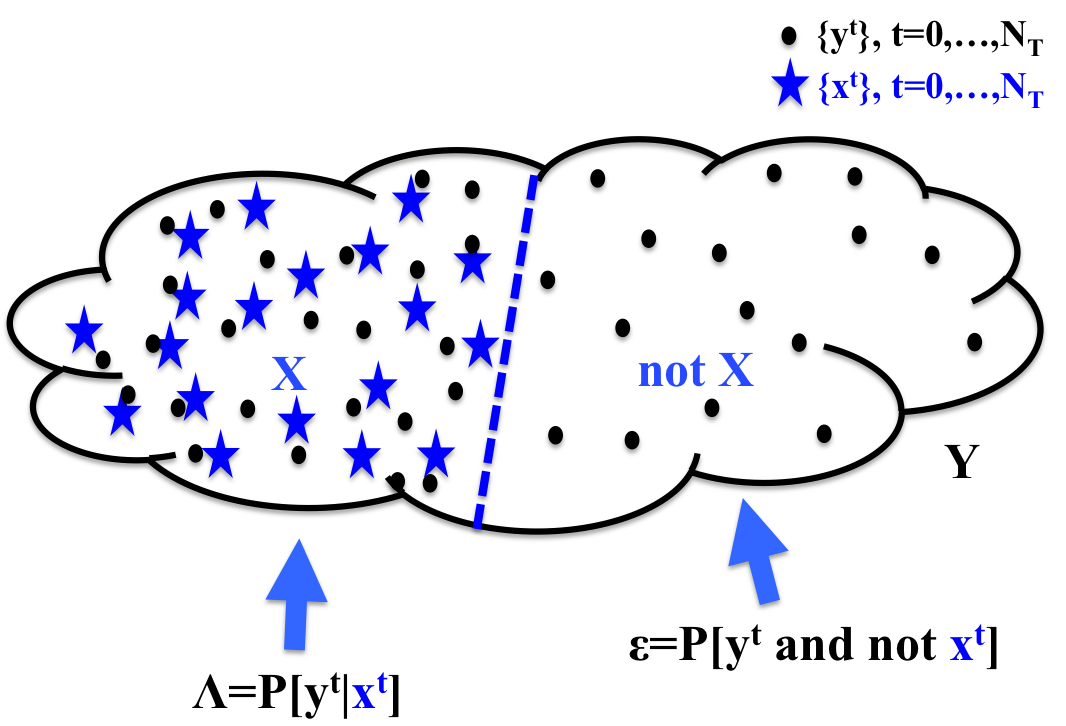
\includegraphics[width=0.35\linewidth, angle=0, clip = true]{figures/Bayesian_Causality_1.png}
%			\hfil
%			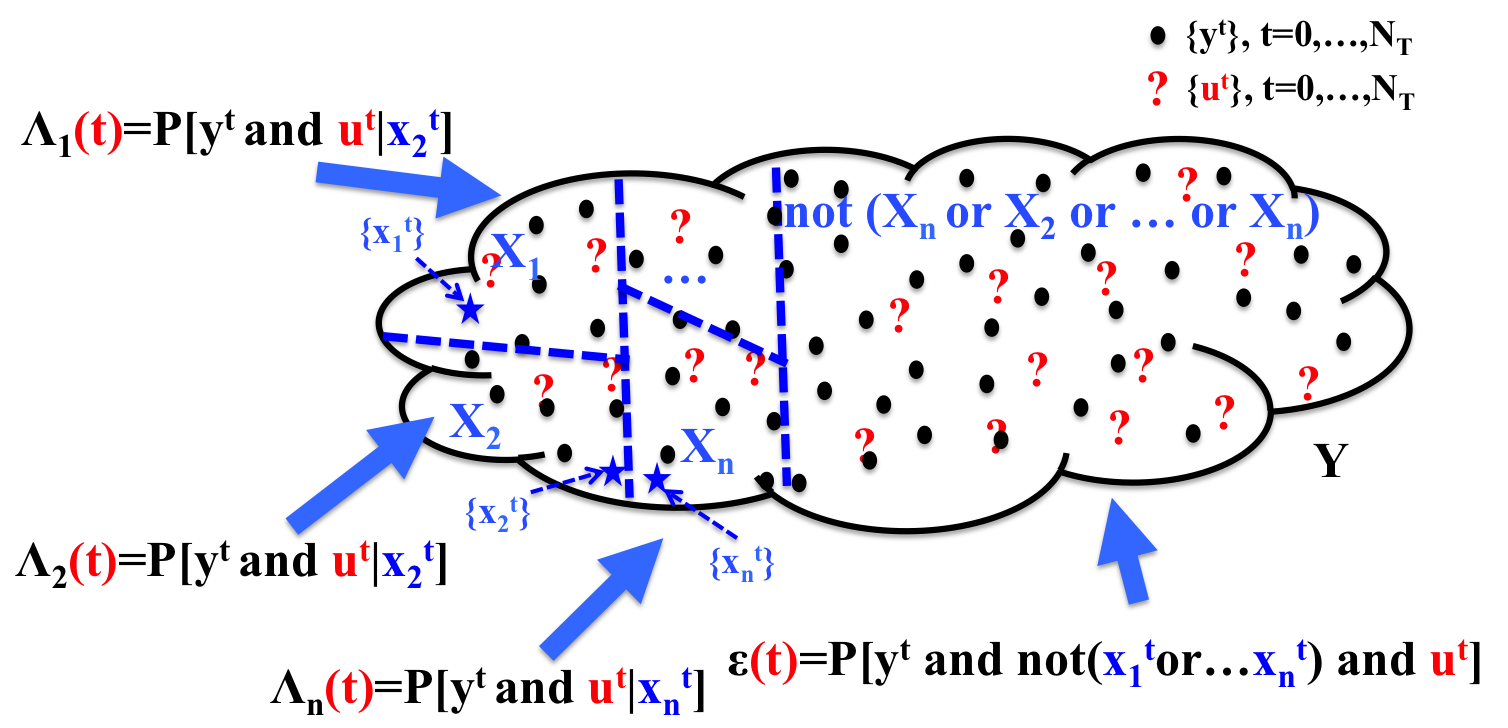
\includegraphics[width=0.55\linewidth, angle=0, clip = true]{figures/Bayesian_Causality_2.png}
%			\caption{The simplest statistical causality model (left) is $P[y^t] = {\bf \Lambda} P[x^t] + \varepsilon$, with $\Lambda \simeq 0$ implying no causality impact of $X$ on $Y$.  The law of total probability  allows a partition (right):  $P[y^t \hat u^t] = \Lambda_1(t) P[x_1^t] + \Lambda_2(t) P[x_2^t]  + \ldots + \Lambda_n(t) P[x_n^t]$, with  $\Lambda_i \simeq 0$ implying no causality impact of  $X_i$ on $Y$.}
%		\end{center}
%	\end{figure}
%\end{column}	
%\begin{column}{0.05\linewidth}\end{column}
%\end{columns}

%\vskip2ex
%\end{block}


%----------------------------------------------------------------------------------------
%	Algorithm:  approximation through well-posed lower bound
%----------------------------------------------------------------------------------------

\begin{block}{Algorithm:  approximation through well-posed lower bound}

Assuming $y^t$ being statistically-independent in $t$  sequence of binary variables or observed probabilities 
(conditioned on the knowledge of variables $x$ and $u$), inference of both the unknown causality vector $\Lambda(t)$ 
and of the unknown probability process $P_y^t$ for the discrete state model  
\begin{displaymath}
P_y^t = \Lambda^{\dagger}(t)P^t_x,
\end{displaymath}
can be done via a maximisation 
w.r.t.~$\Lambda(t)$ of the following log-likelihood functional:

\begin{equation}
\label{eq:loglik}
\mathcal{L}=\max_{\Lambda} \left( \sum_{t=0}^{N_T}\left[\left(1-y^t\right)\ln\left(1-\Lambda^{\dagger}(t)P_x^t\right)
+y^t\ln\left(\Lambda^{\dagger}(t)P^t_x\right)\right] \right).
\end{equation}

\noindent This problem is unfortunately ill-posed.  The central challenge is to formulate the investigations of $\Lambda_i$ 
into a well-posed optimisation problem.  We start with the approximation:

$$\Lambda (t) = \sum_{i=1}^{K} \gamma_i^t \Lambda_i \;\; \mbox{with} \;\; \sum_{i=1}^K \gamma_i^t = 1, \;\; \gamma_i^t \ge 0.$$

\noindent In \cite{horenko_pnas_2014} the following lower bound for $\mathcal{L}$ was proved:

\begin{equation}
\label{eq:loglik_lb}
%\begin{multlined}
\mathcal{L} \ge l^\epsilon= \max_{\gamma_i^t,\Lambda_i} \left( \sum_{i=1}^{\mathbf{K}}\left[\sum_{t=0}^{N_T}\gamma^t_i g\left(t,\Lambda_i\right)-\epsilon^2\sum_{j=1}^n\lambda_{i}^{(j)}\right] \right).
%\end{multlined}
\end{equation}

\noindent with 
% TODO: $g\left(t,\Lambda_i\right)=\left(1-y^t\right)\ln\left(1-\Lambda^{\dagger}_iP_x^t\right)+y^t\ln\left(\Lambda^{\dagger}_iP^t_x\right)$,
and subject to the constraints:

%\begin{eqnarray}
%\label{eq:loglik_lb_con00}
%&& \sum_{i=1}^{\mathbf{K}}\gamma_i^t=1,  \gamma_i^t\geq 0 \text{ for all $t$ and $i$,}\\
%\label{eq:loglik_lb_con0}
%&&0<\sum_{j=1}^n\lambda_{i}^{(j)}< 1,\quad  0\leq\lambda_{i}^{(j)}\leq1, \text{ for all $i$ and $j$,}\\
 %\label{eq:loglik_lb_con}
% &&\sum_{t_1,t_2=0}^{N_T}|\gamma_i^{t_1}-\gamma_i^{t_2}|\leq\bar{\mathbf{C}}\left(N_T\right) ,\text{ for all $i$.}
%\end{eqnarray}

\begin{equation}
\label{eq:loglik_lb_con}
 \sum_{i=1}^{\mathbf{K}}\gamma_i^t=1,  \gamma_i^t\geq 0 \text{ for all $t$ and $i$,} ~~
 0<\sum_{j=1}^n\lambda_{i}^{(j)}< 1,\quad  0\leq\lambda_{i}^{(j)}\leq1, \text{ for all $i$ and $j$,} ~~
 \sum_{t_1,t_2=0}^{N_T}|\gamma_i^{t_1}-\gamma_i^{t_2}|\leq\bar{\mathbf{C}}\left(N_T\right) ,\text{ for all $i$.}
\end{equation}


\noindent The maximisation of $l^\epsilon$ belongs to the well-posed class of FEM-BV-problems.

\end{block}


%----------------------------------------------------------------------------------------
%	High Performance Computing Implementation
%----------------------------------------------------------------------------------------

\begin{block}{High Performance Computing Implementation}

We start the development of our new HPC Causality library implementing more simplier models. 
The Granger Causality could be used for modelling general whole set of non-stationary models solving the general optimisation problem
with \emph{average cluster functional}
\begin{equation}
 \label{eq:general}
 L(\theta_1, \dots, \theta_K, \Gamma) 
 = \sum\limits_{t = m}^{T} \sum\limits_{k = 1}^{K} \gamma_k^t g(x^t,\dots,x^{t-m}, \theta_k) ~~ \rightarrow \min
\end{equation}
where $\theta_k$ represents parameters of the model on $k$-th cluster (unknown)
and $\gamma_k$ are \emph{model indicator functions} (unknown). These functions represent the presence
of appropriate model on $k$-th cluster. The error of the model on $k$-th cluster is computed via \emph{model error functions} $g$.
For complete review and applications see Metzner et. al \cite{metzner_2012}. 
Also presented problem \eqref{eq:loglik} could be considered as a special case of optimisation problem \eqref{eq:general}.
The nonconvex problem \eqref{eq:general} could be solved iteratively as a sequence of solution of two optimisation problems, see Algorithm \ref{alg:outer}.

\begin{columns}[T]
\begin{column}{0.02\linewidth}\end{column}

\begin{column}{0.4\linewidth}
	\begin{center}
	\begin{table}[h!]
	\renewcommand{\tablename}{Algorithm}
	\fbox{\it
	\begin{tabular}{p{0.95\linewidth}}
	\medskip
	\hspace*{0.6CM}set feasible initial approximation $\Gamma_{0}$\\
	\medskip
	\hspace*{0.6CM}{\textbf{while}} $\Vert L(\Gamma_{it},\Theta_{it}) - L(\Gamma_{it-1},\Theta_{it-1}) \Vert \geq \varepsilon$\\
	\hspace*{1.2CM} solve $\Theta_{it} = \arg \min\limits_{\Theta} L(\Theta, \Gamma_{it-1})$ $~~~$ (with fixed $\Gamma_{it-1}$) \\
	\hspace*{1.2CM} solve $\Gamma_{it} = \arg \min\limits_{\Gamma} L(\Theta_{it}, \Gamma)$ $~~~$ (with fixed $\Theta_{it}$) \\
	\hspace*{1.2CM} $it = it + 1$ \\
	\hspace*{0.6CM}{\textbf{endwhile}} \\
	\medskip
	\end{tabular}
	}
	\caption{\label{alg:outer} \bf Outer algorithm.}
	\end{table}
	\end{center}

	\vskip2ex
	
	\begin{equation}
	\label{eq:qp}
	\begin{array}{c}
		\Gamma_{it} = \arg\min \frac{1}{2} \gamma^T H \gamma + g^T \gamma \\[1ex]
		\textrm{subject to} ~~~ \forall t: \sum\limits_{k=1}^{K} \gamma_{k}^t = 1, \gamma \geq 0.
	\end{array}
	\end{equation}	
		
	\vskip3ex
	
	\begin{equation}
	 \label{eq:aic}
	 AIC(L,\Theta,K) = - 2 \ln L + 2 (\textrm{sizeof}(\Theta) + K)
	\end{equation}
\end{column}	

\begin{column}{0.54\linewidth}
	\begin{center}
	\begin{table}[h!]
	\renewcommand{\tablename}{Algorithm}
	\fbox{\it
	\begin{tabular}{p{1.0\linewidth}}
	Given initial approximation $x^{0} \in \Omega$, 
	parameters $m \in \mathbb{N}, \gamma \in (0,1)$, \\
	safeguarding parameter $\sigma_2 \in (0, 1)$, and initial step-size $\alpha_0 > 0$. \medskip \\
	\hspace*{1.2CM} $k := 0$\\
	\hspace*{1.2CM} $g^0 := Ax^0 - b$\\
	\hspace*{1.2CM} $f^0 := 1/2 \langle g^0 - b, x^0 \rangle$ \medskip \\
	\hspace*{1.2CM} {\textbf{while}} $\Vert \widetilde{g}_{\alpha}(x) \Vert$ is not sufficiently small \\
	\hspace*{1.7CM} $d^k := P(x^k - \alpha_k g^k) - x^k$  \medskip\\
	\hspace*{1.7CM} $f_{\max} := \max \lbrace f(x^{k-j}): 0 \leq j \leq \min \lbrace k,m-1 \rbrace \rbrace$ \\
	\hspace*{1.7CM} $\xi := (f_{\max} - f^k) / \langle A d^k, d^k \rangle$ \\
	\hspace*{1.7CM} $\bar{\beta} := - \langle g^k, d^k \rangle / \langle A d^k, d^k \rangle$ \\ 
	\hspace*{1.7CM} $\hat{\beta} := \gamma \bar{\beta} + \sqrt{\gamma^2\bar{\beta}^2 + 2 \xi}$ \\ 
	\hspace*{1.7CM} choose $\beta_k \in [ \sigma_1, \min \lbrace \sigma_2, \hat{\beta} \rbrace ]$ \medskip \\ 
	\hspace*{1.7CM} $x^{k+1} := x^k + \beta_k d^k$\\
	\hspace*{1.7CM} $g^{k+1} := g^k + \beta_k A d^k$\\
	\hspace*{1.7CM} $f^{k+1} := 1/2 \langle g^{k+1} - b, x^{k+1} \rangle$  \medskip\\
	\hspace*{1.7CM} $\alpha_{k+1} := \langle d^k, d^k \rangle / \langle Ad^k, d^k \rangle$ \medskip\\
	\hspace*{1.7CM} $k := k + 1$ \\
	\hspace*{1.2CM} {\textbf{endwhile}} \\
	\smallskip
	Return approximation of solution $x^k$.
	\end{tabular}
	}
	\caption{\label{alg:spg_qp} \bf Spectral projected gradient method for QP (SPG-QP).}
	\end{table}
	\end{center}
\end{column}	
\begin{column}{0.02\linewidth}\end{column}
\end{columns}

\end{block}

%----------------------------------------------------------------------------------------
%	Acknowledgements
%----------------------------------------------------------------------------------------


\begin{block}{Acknowledgements}

\noindent
\par 

This work is supported by Platform for Advanced Scientific Computing (PASC).
We would like to thank Olga Kaiser, Dimitri Igdalov, Ganna Marchenko, Ben Cumming, and Patrick Sanan for their collaboration in the project.

%\vskip2ex
\end{block}

%----------------------------------------------------------------------------------------

\end{column} % End of the first column


\begin{column}{.02\textwidth}\end{column} % Empty spacer column

 
\begin{column}{.48\textwidth} % The second column

%----------------------------------------------------------------------------------------
%	QP
%----------------------------------------------------------------------------------------

\begin{block}{Quadratic Programming problem}

Please notice that the second problem (i.e. $\Gamma$-problem) is independent on selected model. The model indicator functions $\Gamma$ are represented by vector of dimension $K \cdot T$
have to fullfill conditions \eqref{eq:loglik_lb_con} with so-called BV norm. However, instead of 
using BV-norm, we can use Euclidean norm and appropriate FEM regularisation, see Horenko \cite{horenko_fem}. The obtained optimisation problem is Quadratic Programming problem
with SPS Hessian matrix and feasible set defined by simplex \eqref{eq:qp}. Solving this problem is the most time-consuming operation.

In our library, we are using a Spectral Projected Gradient method (see Martinez et al. \cite{spg}) simplified for QP problems (see Algorithm \ref{alg:spg_qp}) developed by Pospisil \cite{pospisil_phd}.
The algorithm is based on the solving the sequence of projection problems and since the feasible set is described by separable simplex constraints (of dimension $K$),
this system extends the granularity of the solution process and it is suitable for GPU.

\begin{columns}[T]
\begin{column}{0.02\linewidth}\end{column}
\begin{column}{0.94\linewidth}
	\begin{figure}[H]
		\begin{center}
			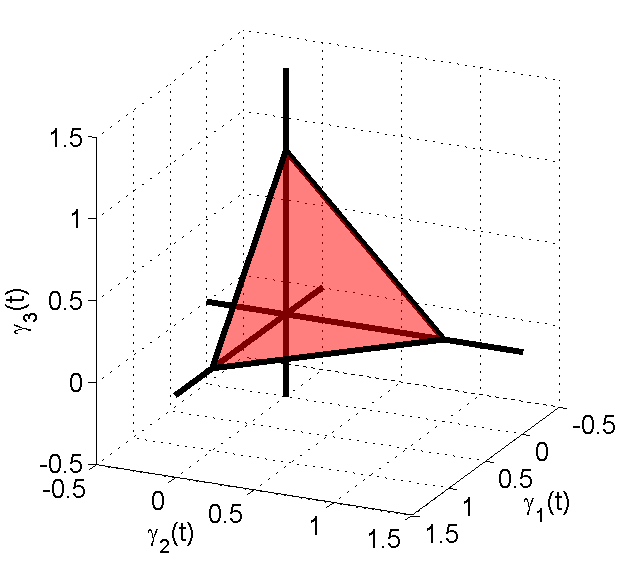
\includegraphics[width=0.3\linewidth, angle=0, clip = true]{figures/simplex.png}
			\hfil
			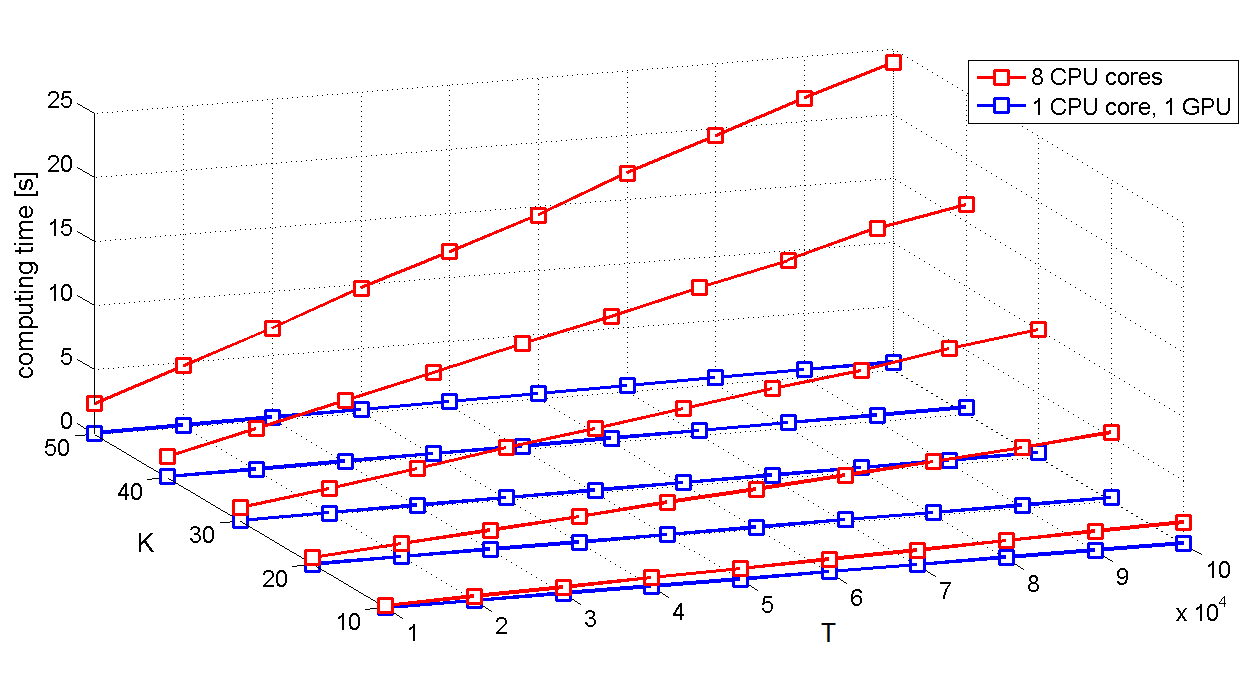
\includegraphics[width=0.5\linewidth, angle=0, clip = true]{figures/projection.png}
			\caption{Projection onto feasible set: the feasible set in Quadratic Programming problem ($\Gamma$-problem in Algorithm \ref{alg:outer}) consists of 
			separable simplexes; example for $K=3$ is presented on left figure.
			We solve the problem of projection onto simplex using algorithm presented by Chen and Ye \cite{simplex}. The number of iterations of this algorithm is upper bounded by $K$.
			Right figure shows the computing time of $100$ random vectors of length $K \cdot T$ using one node on PIZ Daint machine (Intel® Xeon® E5-2670 (8 cores, 32GB) with NVIDIA® Tesla® K20X (2688 cores, 6GB)).
			}
		\end{center}
	\end{figure}
\end{column}	
\begin{column}{0.02\linewidth}\end{column}
\end{columns}

\end{block}



\begin{block}{Parallelisation}
Since the number of clusters $K$ and the memory parameters $p,q$ in model \eqref{eq:ARX} are unknown, the optimization problem \eqref{eq:general}
with different choice of these parameters has to be solved. Also different choise of initial $\Gamma_0$ leads to different results.
These problems are completely independent and leads to the straightforward parellelisation. In the end of solution process, the solution with the lowest AIC number \eqref{eq:aic}
is chosen as a solution of the original problem. \newline

At the beginning of our implementation, we focus on more complicated problem. We suppose that the original data of time series are such large that it cannot be stored
and operated on one node with shared memory, see Figure \ref{fig:parallelisation}. 
However, the data of inner optimisation problems ($\Gamma$-problem and $\Theta$-problem) have to be assembled in each outer iterations from data of time-series.
Therefore, the communication (scattering of time-series) has to be handled.
Our first implementation supposes that inner optimisation problems have still such a small dimension to be solved on one processor (and/or on one GPU card).

\begin{columns}[T]
\begin{column}{0.02\linewidth}\end{column}
\begin{column}{0.94\linewidth}
	\begin{figure}[H]
		\begin{center}
			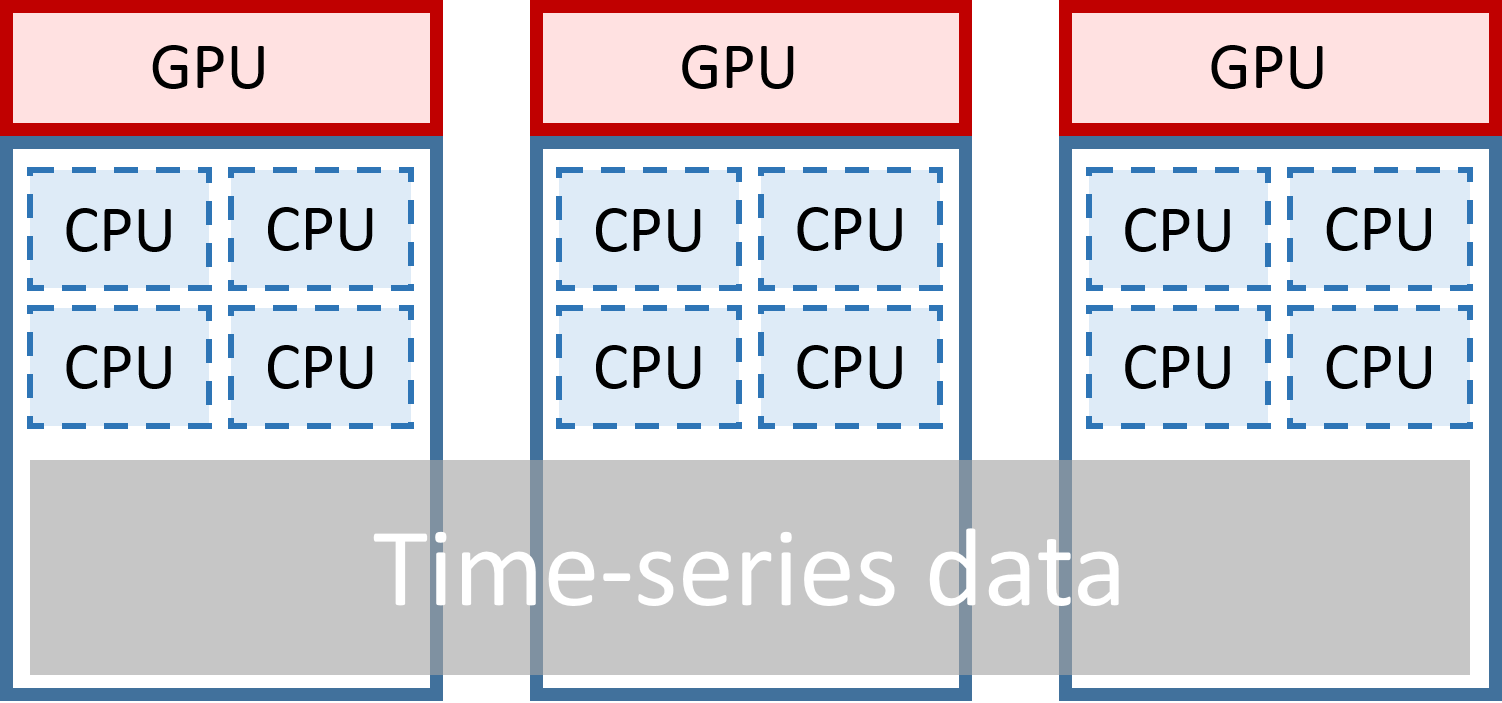
\includegraphics[width=0.22\linewidth, angle=0, clip = true]{figures/computing_node.png}
			\hfil
			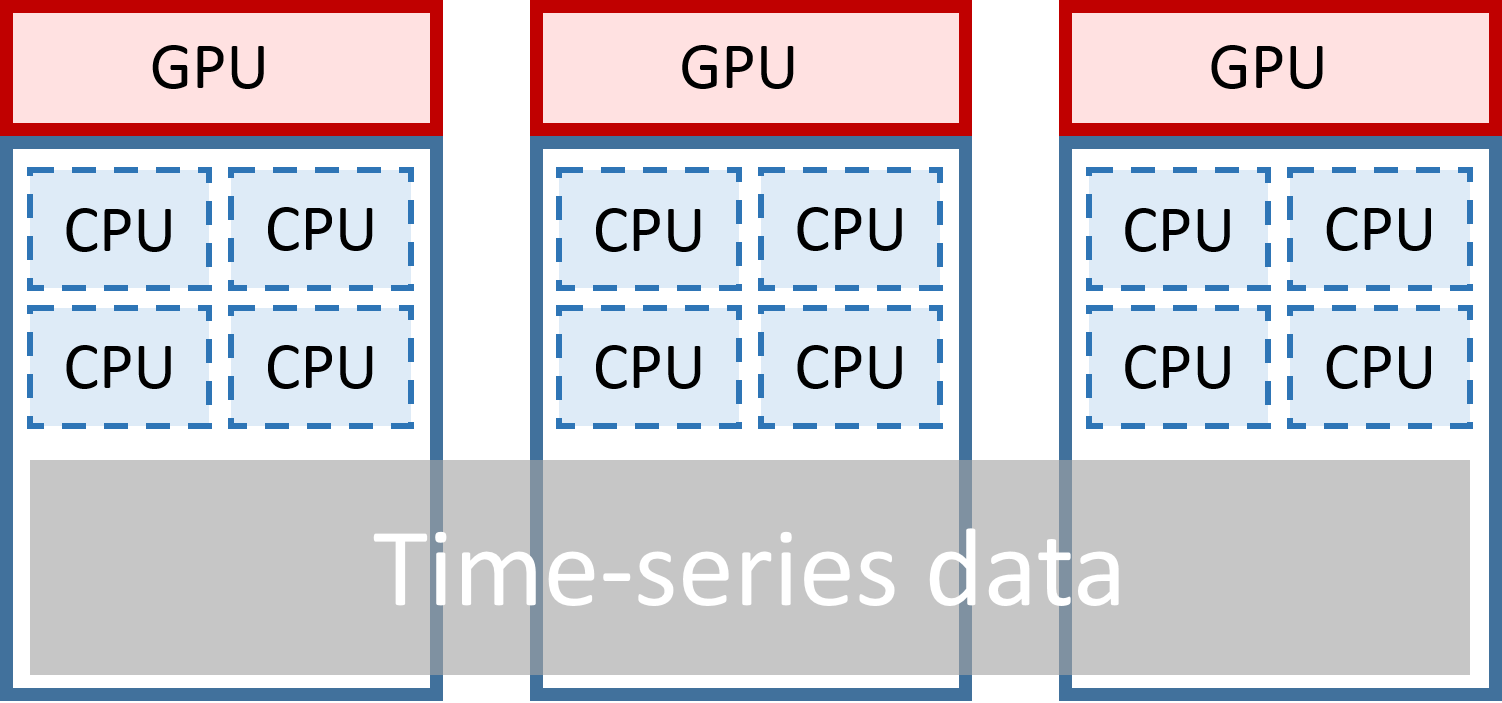
\includegraphics[width=0.22\linewidth, angle=0, clip = true]{figures/computing_node.png}
			\hfil
			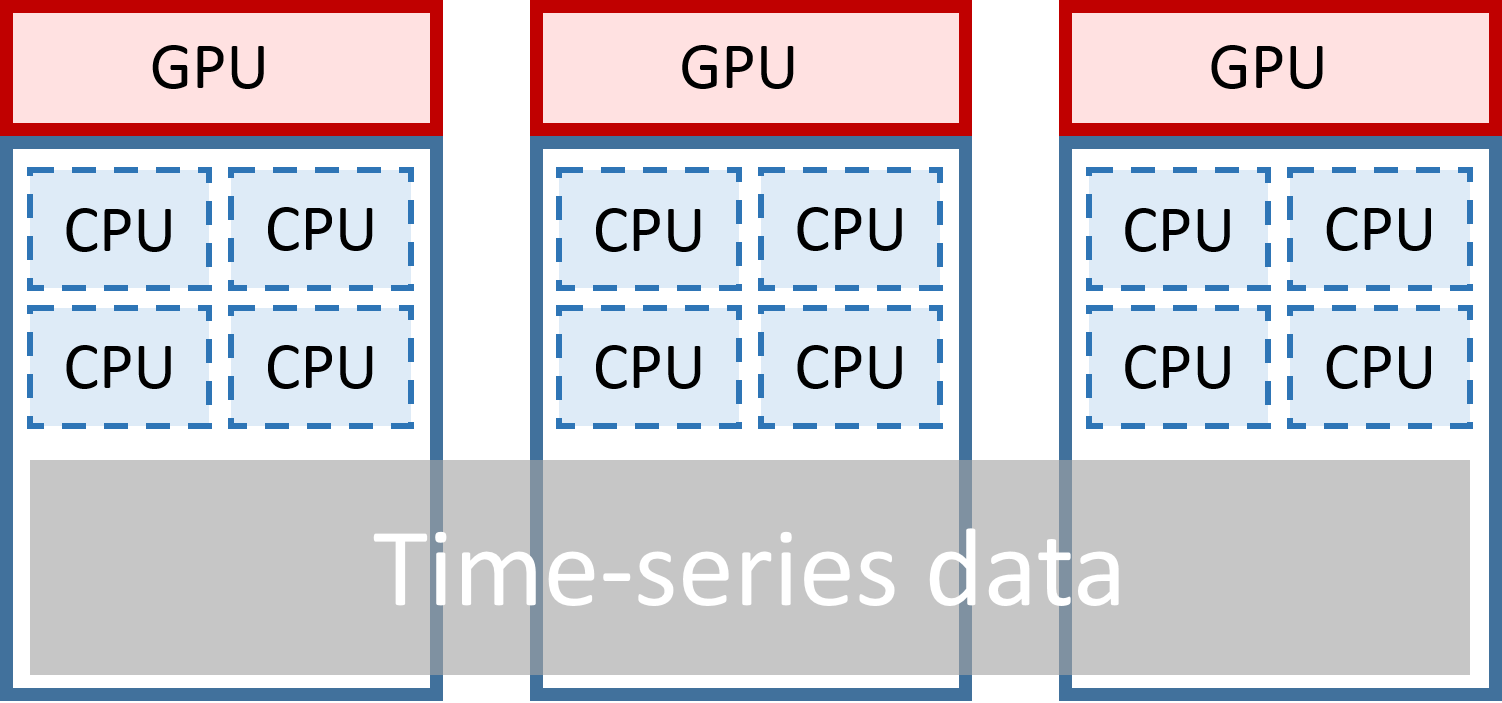
\includegraphics[width=0.22\linewidth, angle=0, clip = true]{figures/computing_node.png}
			\hfil
			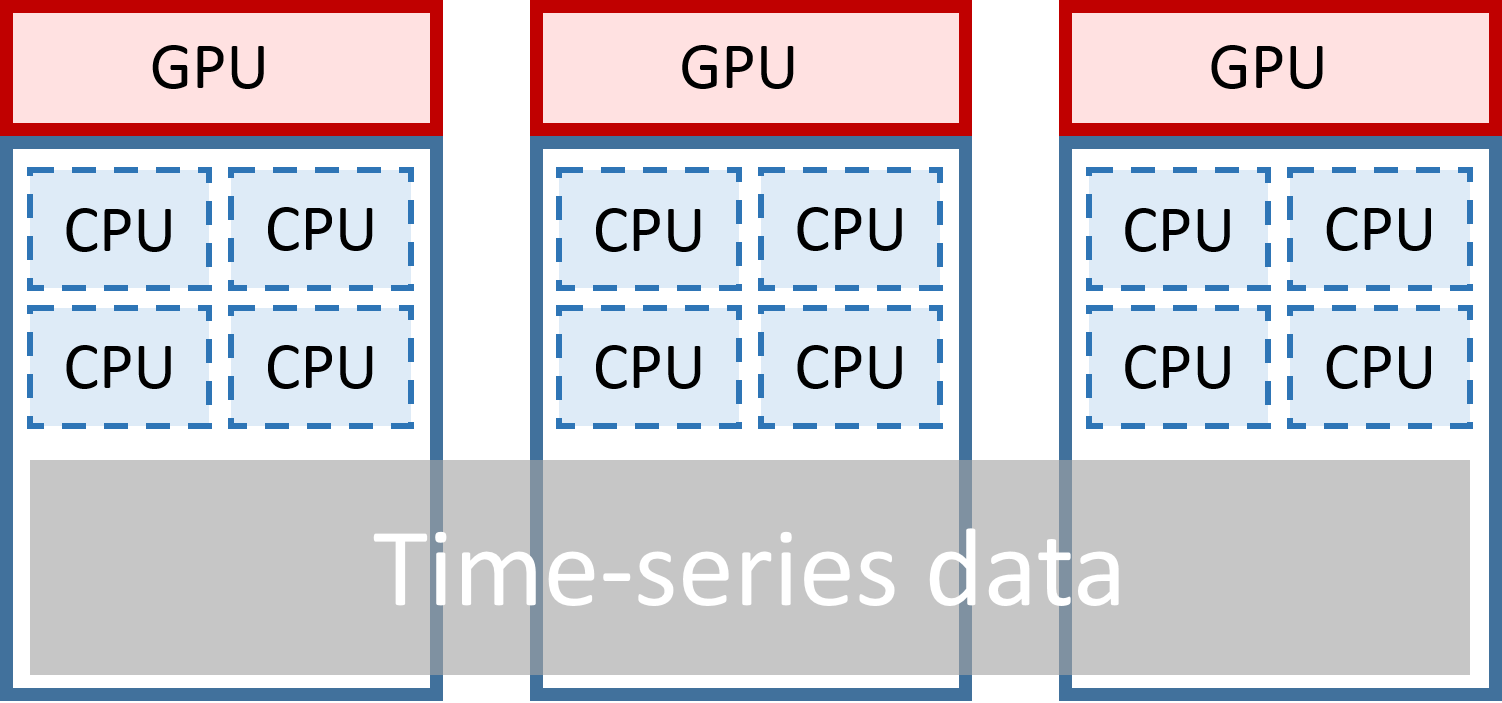
\includegraphics[width=0.22\linewidth, angle=0, clip = true]{figures/computing_node.png}
			\caption{Computation on large-scale time-series data. We suppose that the data of time-series cannot be operated on one single node, therefore the communication is necessary.
					 However, each node is still solving its own problem with given parameters.
					 }
			\label{fig:parallelisation}		 
		\end{center}
	\end{figure}
\end{column}	
\begin{column}{0.02\linewidth}\end{column}
\end{columns}

\vskip2ex

In furture work, we create a management on the top of this approach. Each computing unit will consist of the set of nodes operating together on one data vector, but still
each node will be able to compute its own optimisation problem with given $K$ and given initial approximation $\Gamma_{0}$. Actual implementation consist of only one computing node,
therefore in this time, we are still able to solve the problems on large data sets sending a independent computing jobs on supercomputer.

\end{block}

\begin{block}{Numerical experiments -  Geometrical clustering with Kmeans model} 

Geometrical clustering problem represents the most basic modelling functions - constant function. 
We are trying to model the given data using the one value in every cluster in least-square sence
\begin{displaymath}
 \forall t \in T_k: x^t = \theta_k + \epsilon_t ~~~ 
 L(\theta_1, \dots, \theta_K, \Gamma) 
 = \sum\limits_{t = m}^{T} \sum\limits_{k = 1}^{K} \gamma_k(t) \Vert x^t - \theta_k \Vert^2 ~~ \rightarrow \min 
\end{displaymath}

The early Matlab implementation revealed the main algorithm challenges, see Figure \ref{fig:kmeans_matlab}. The inner problems in Algorithm \ref{alg:outer} could reuse the solution from previous outer iteration
as an initial approximation in new solution process. Moreover, it is not necessary to solve problems exactly and adaptive precision control should be implemented.

\begin{columns}[T]
\begin{column}{0.02\linewidth}\end{column}
\begin{column}{0.94\linewidth}
	\begin{figure}[H]
		\begin{center}
			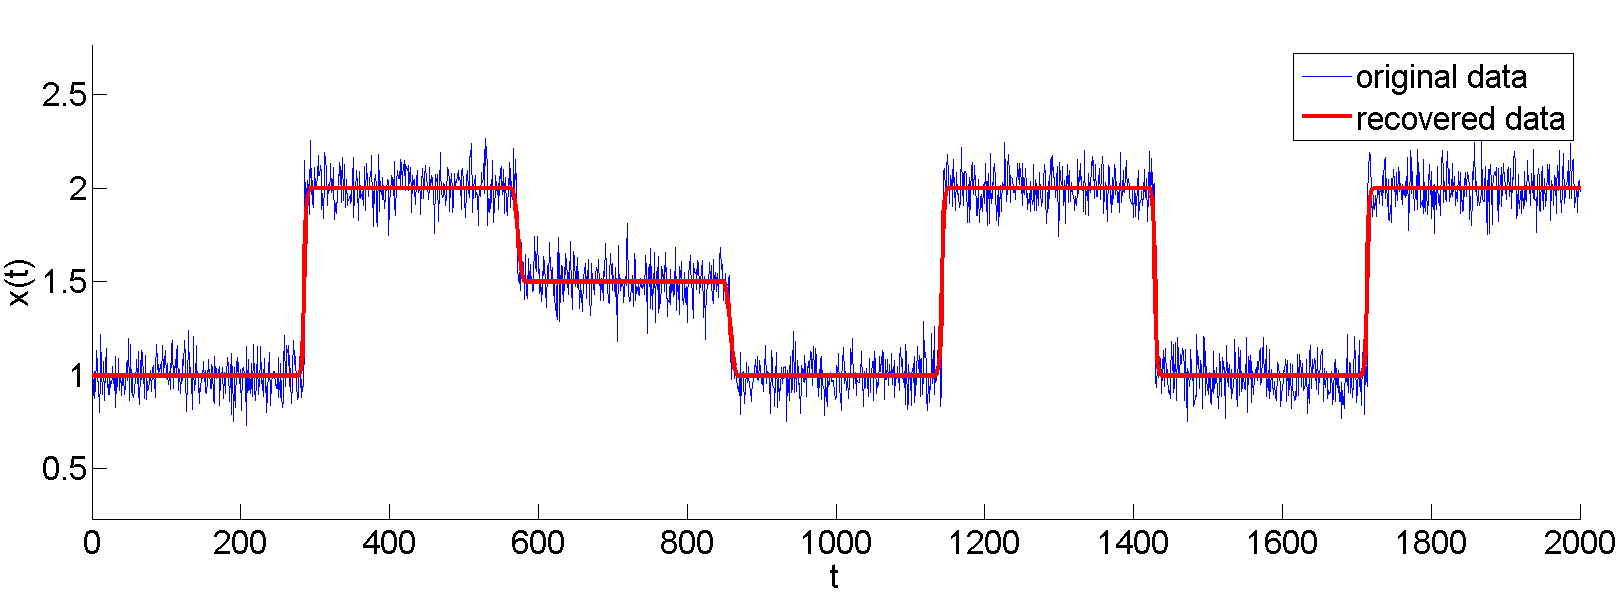
\includegraphics[width=0.49\linewidth, angle=0, clip = true]{figures/kmeans1.png}
			\hfil
			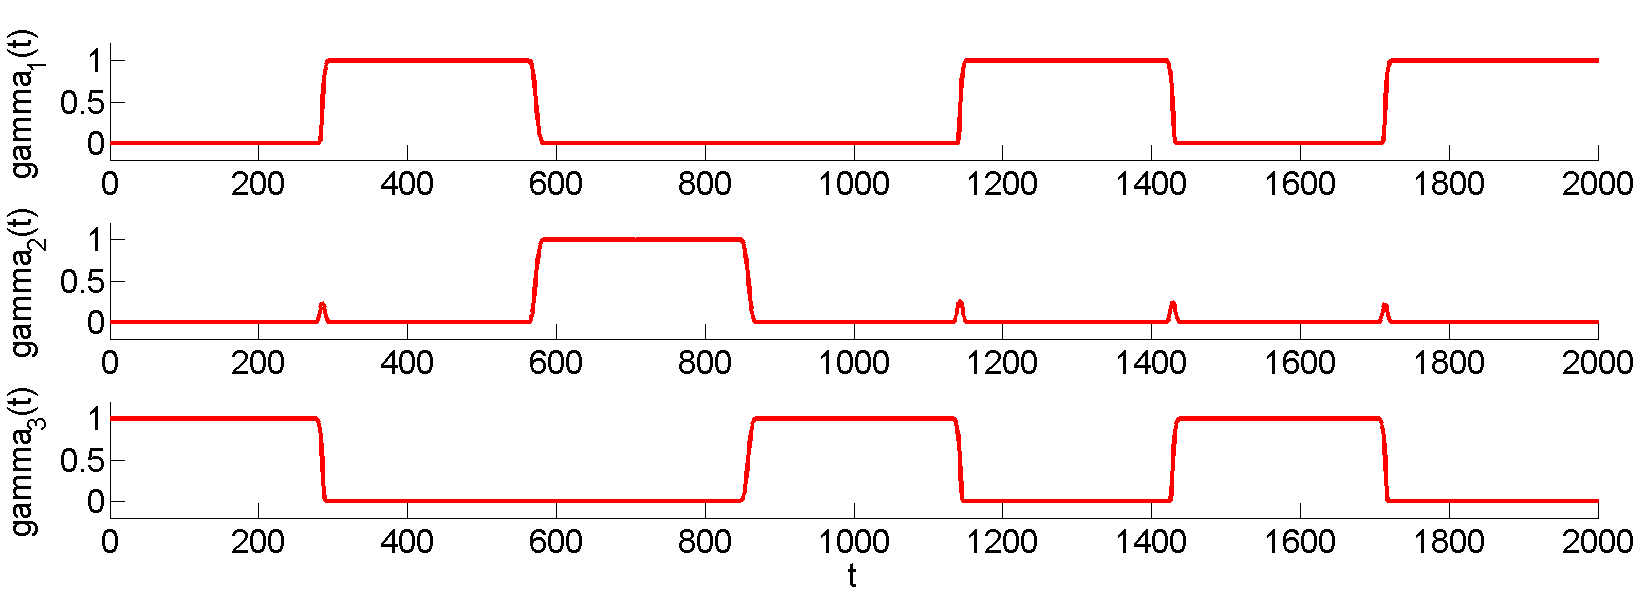
\includegraphics[width=0.49\linewidth, angle=0, clip = true]{figures/kmeans2.png}
			\caption{Initial example: one-dimensional K-means problem with $K=3, T=2000$ solved by FEM-BV-H1 in Matlab. The problem is solved in $4$ outer iterations, the inner QP problem (of dimension $K\cdot N = 6000$) is solved by Matlab \emph{quadprog} solver.
					 Let us remark that the Matlab implementation of \emph{'interior-point-convex'} algorithm is not able to use approximation of solution from previous outer iteration as an initial guess of the solution. Moreover, it is not able to control the precision based on the decrease of the objective function.
					 In projected gradient methods (like SPG-QP), we are able to control the decrease in every iteration as well as use initial approximation.
					 }
			\label{fig:kmeans_matlab}		
		\end{center}
	\end{figure}
\end{column}	
\begin{column}{0.02\linewidth}\end{column}
\end{columns}

\vskip2ex
We implement Algorithm \ref{alg:outer} and Algorithm \ref{alg:spg_qp} in PETSc framework and solve Kmeans problem on 2 nodes on PIZ Daint machine (Intel Xeon E5-2670 (8 cores, 32GB) with NVIDIA Tesla K20X (2688 cores, 6GB))
. The results are presented in Figures \ref{fig:kmeans_pizdaint1}, \ref{fig:kmeans_pizdaint3}, \ref{fig:indicator}, and \ref{fig:L}.
 
\begin{columns}[T]
\begin{column}{0.02\linewidth}\end{column}
\begin{column}{0.46\linewidth}
	\begin{figure}[H]
		\begin{center}
			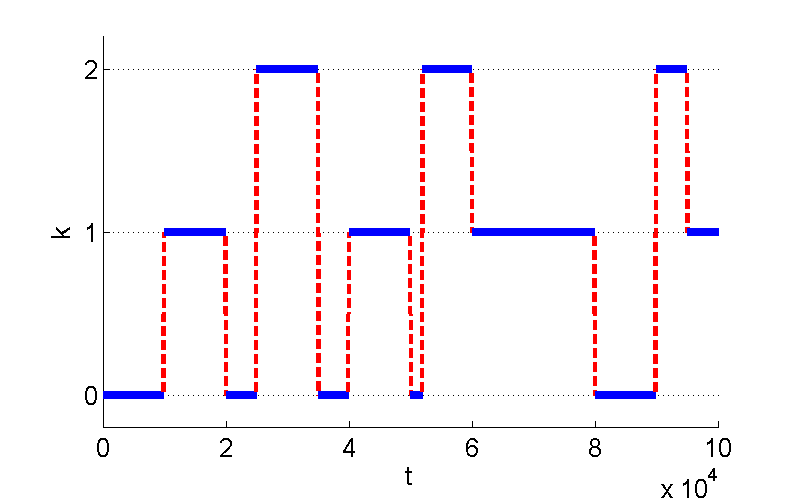
\includegraphics[width=1.0\linewidth, angle=0, clip = true]{figures/generator.png}
			\caption{Large-scaled example: Switching schema for generating testing benchmark.
					 }
			\label{fig:kmeans_pizdaint1}	
		\end{center}
	\end{figure}

	\begin{figure}[H]
		\begin{center}
			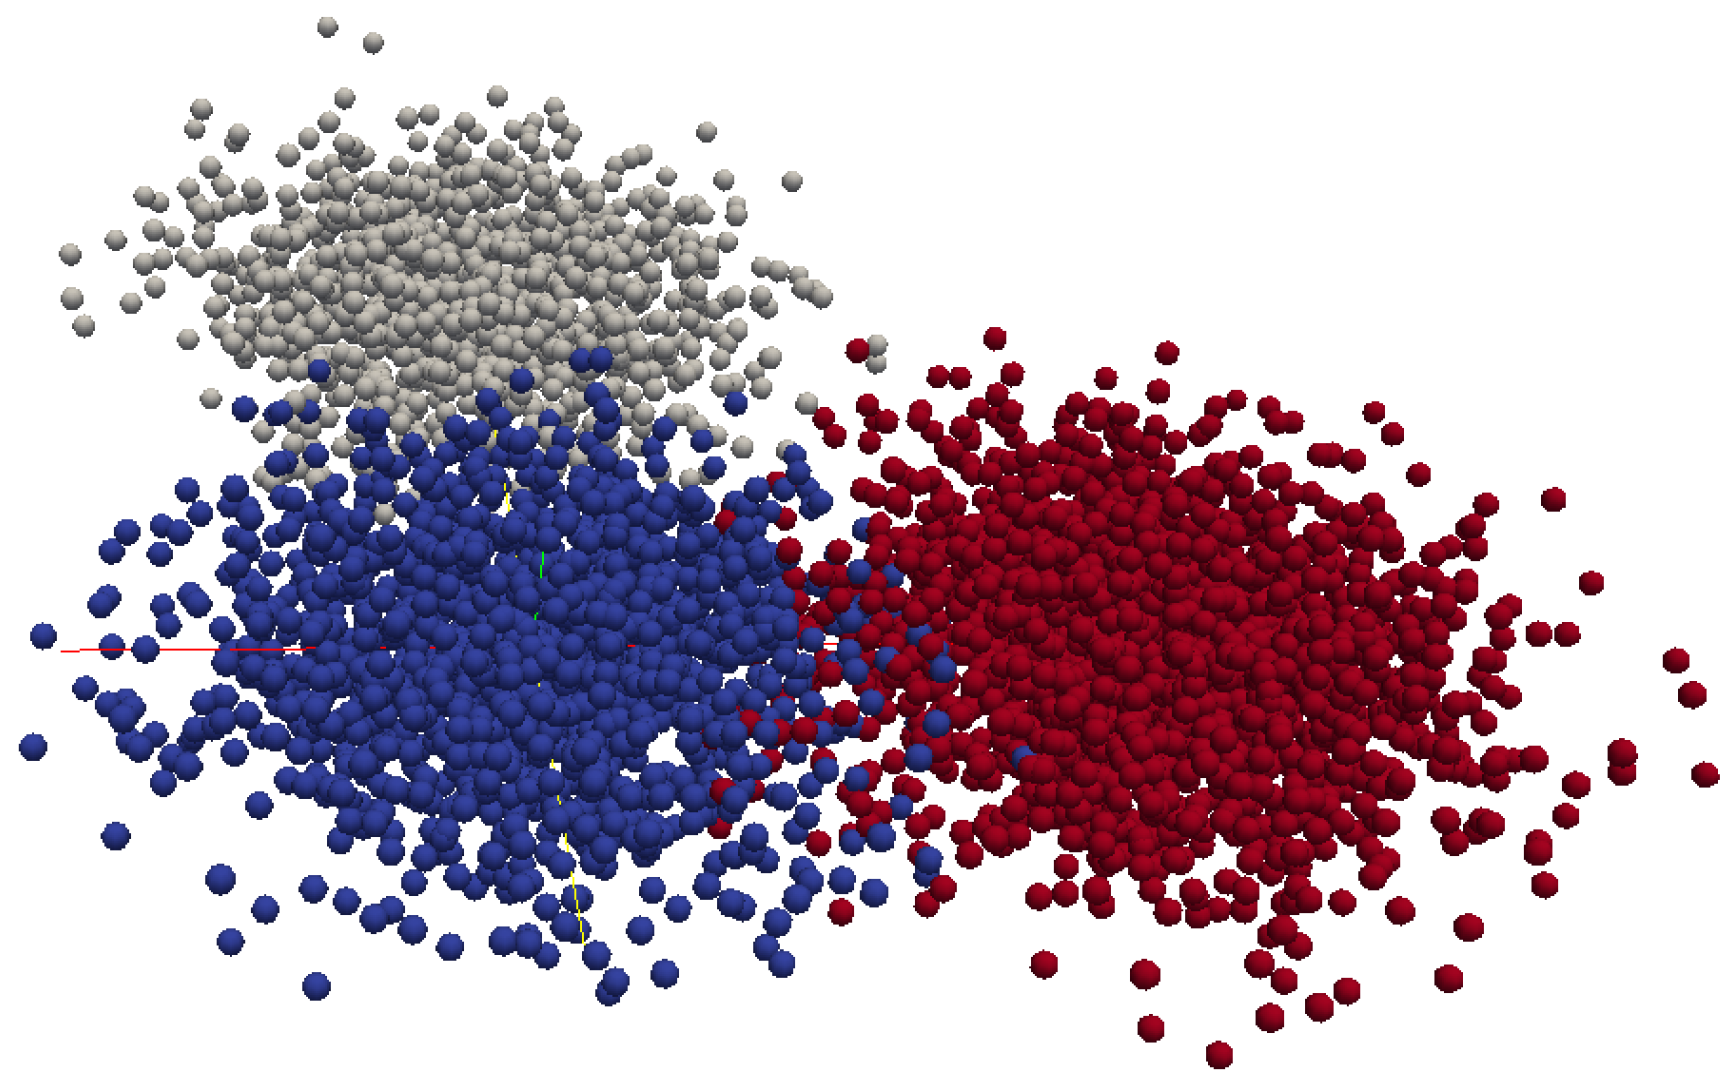
\includegraphics[width=1.0\linewidth, angle=0, clip = true]{figures/solution.png}
			\caption{The solution - clustered data. The affiliation to the cluster is decided by the maximum value of indicator functions $\gamma_0, \gamma_1, \gamma_2$ (see Figure \ref{fig:indicator}). For visualisation, we used VTK format openable in Paraview.
					 }
			\label{fig:kmeans_pizdaint3}	
		\end{center}
	\end{figure}
\end{column}	
\begin{column}{0.02\linewidth}\end{column}
\begin{column}{0.46\linewidth}
	\begin{figure}[H]
		\begin{center}
			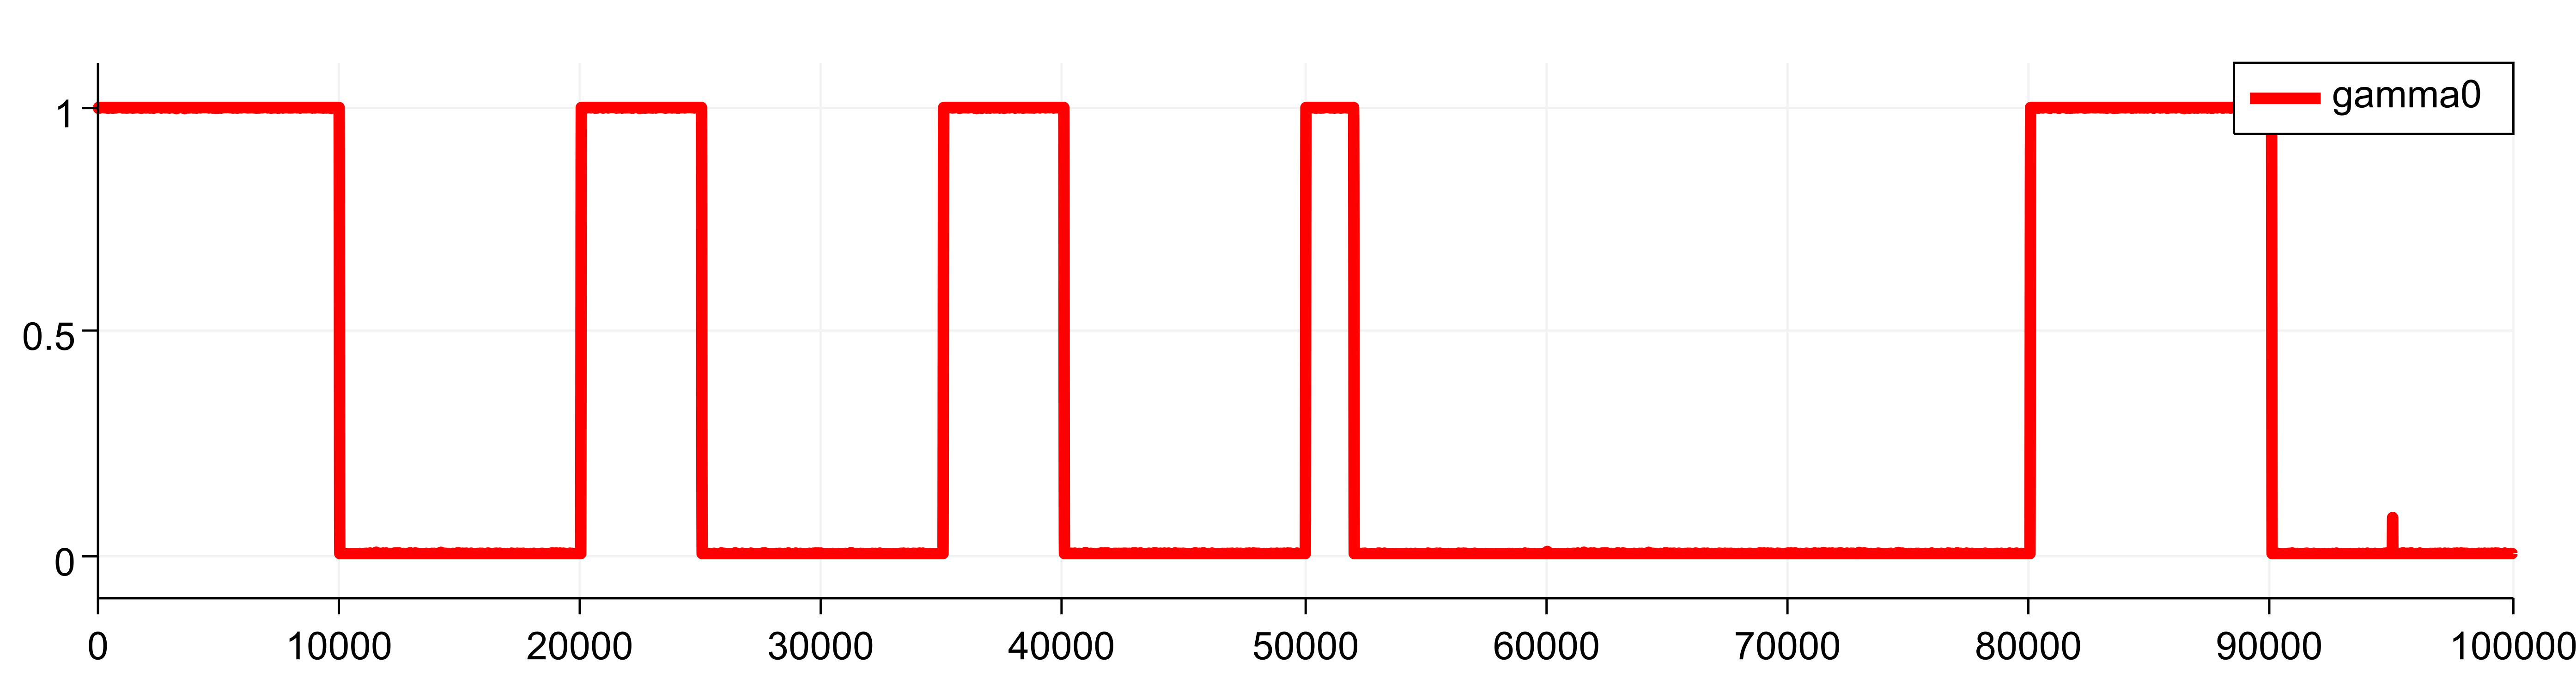
\includegraphics[width=1.0\linewidth, angle=0, clip = true]{figures/gamma0.png} \\
			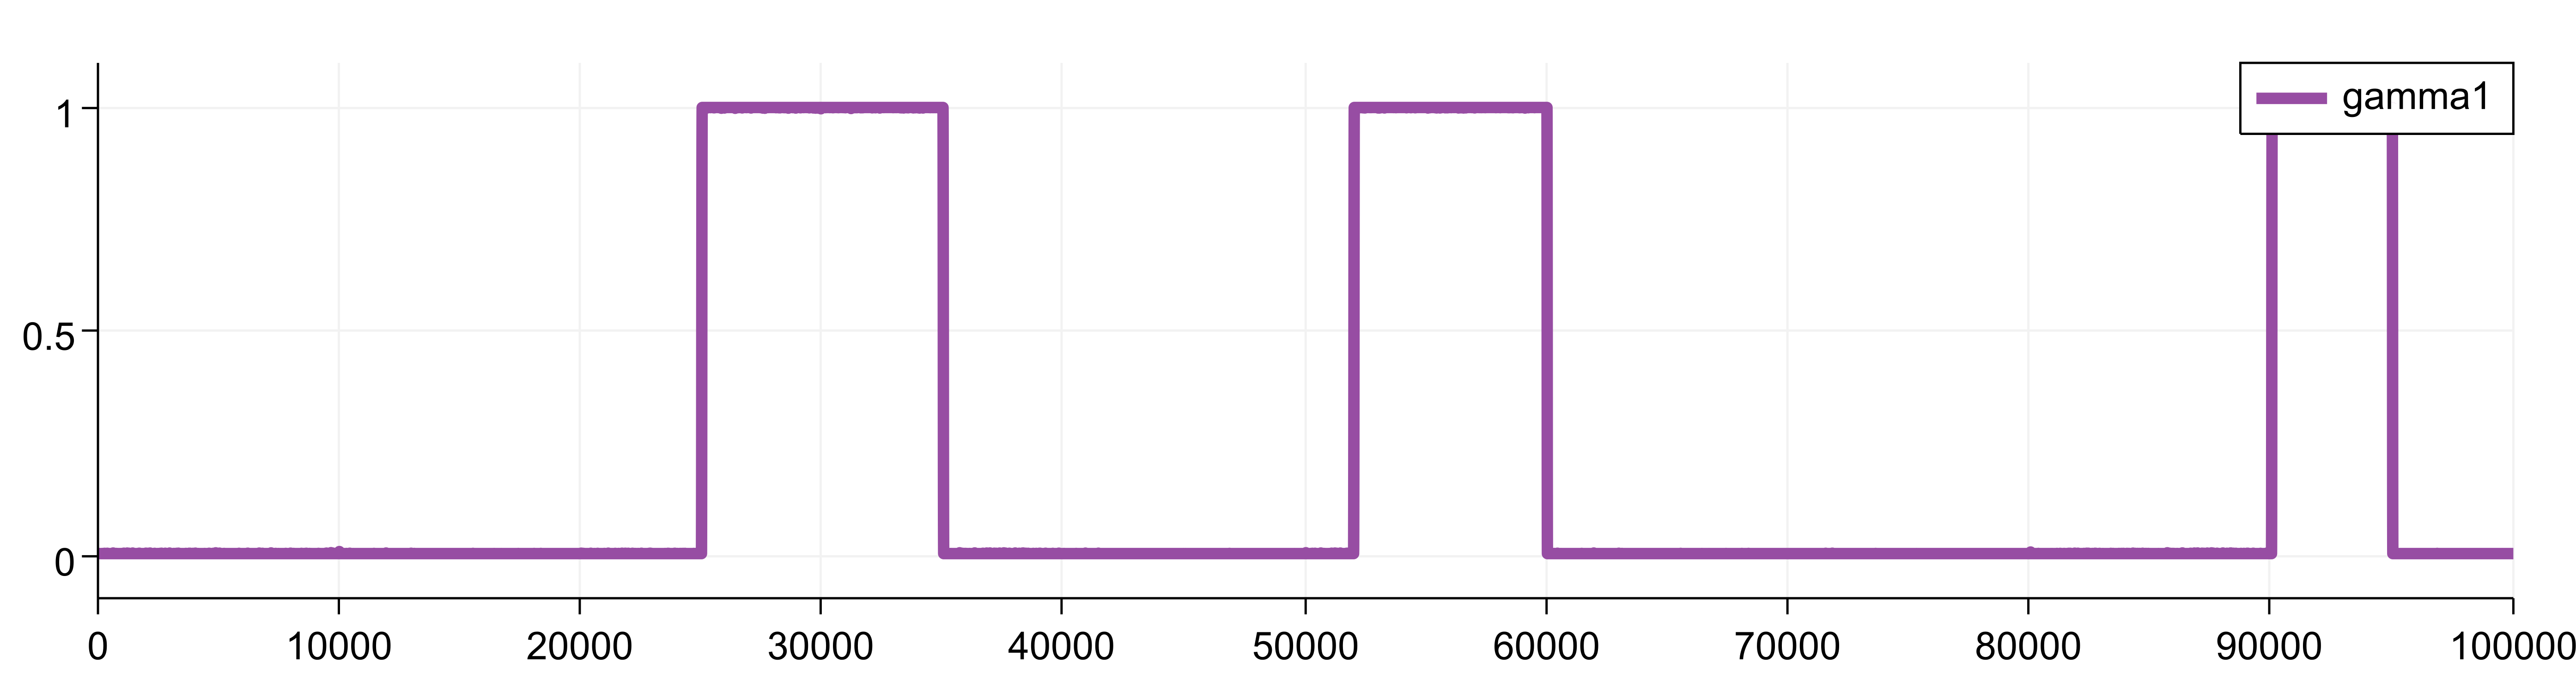
\includegraphics[width=1.0\linewidth, angle=0, clip = true]{figures/gamma1.png} \\
			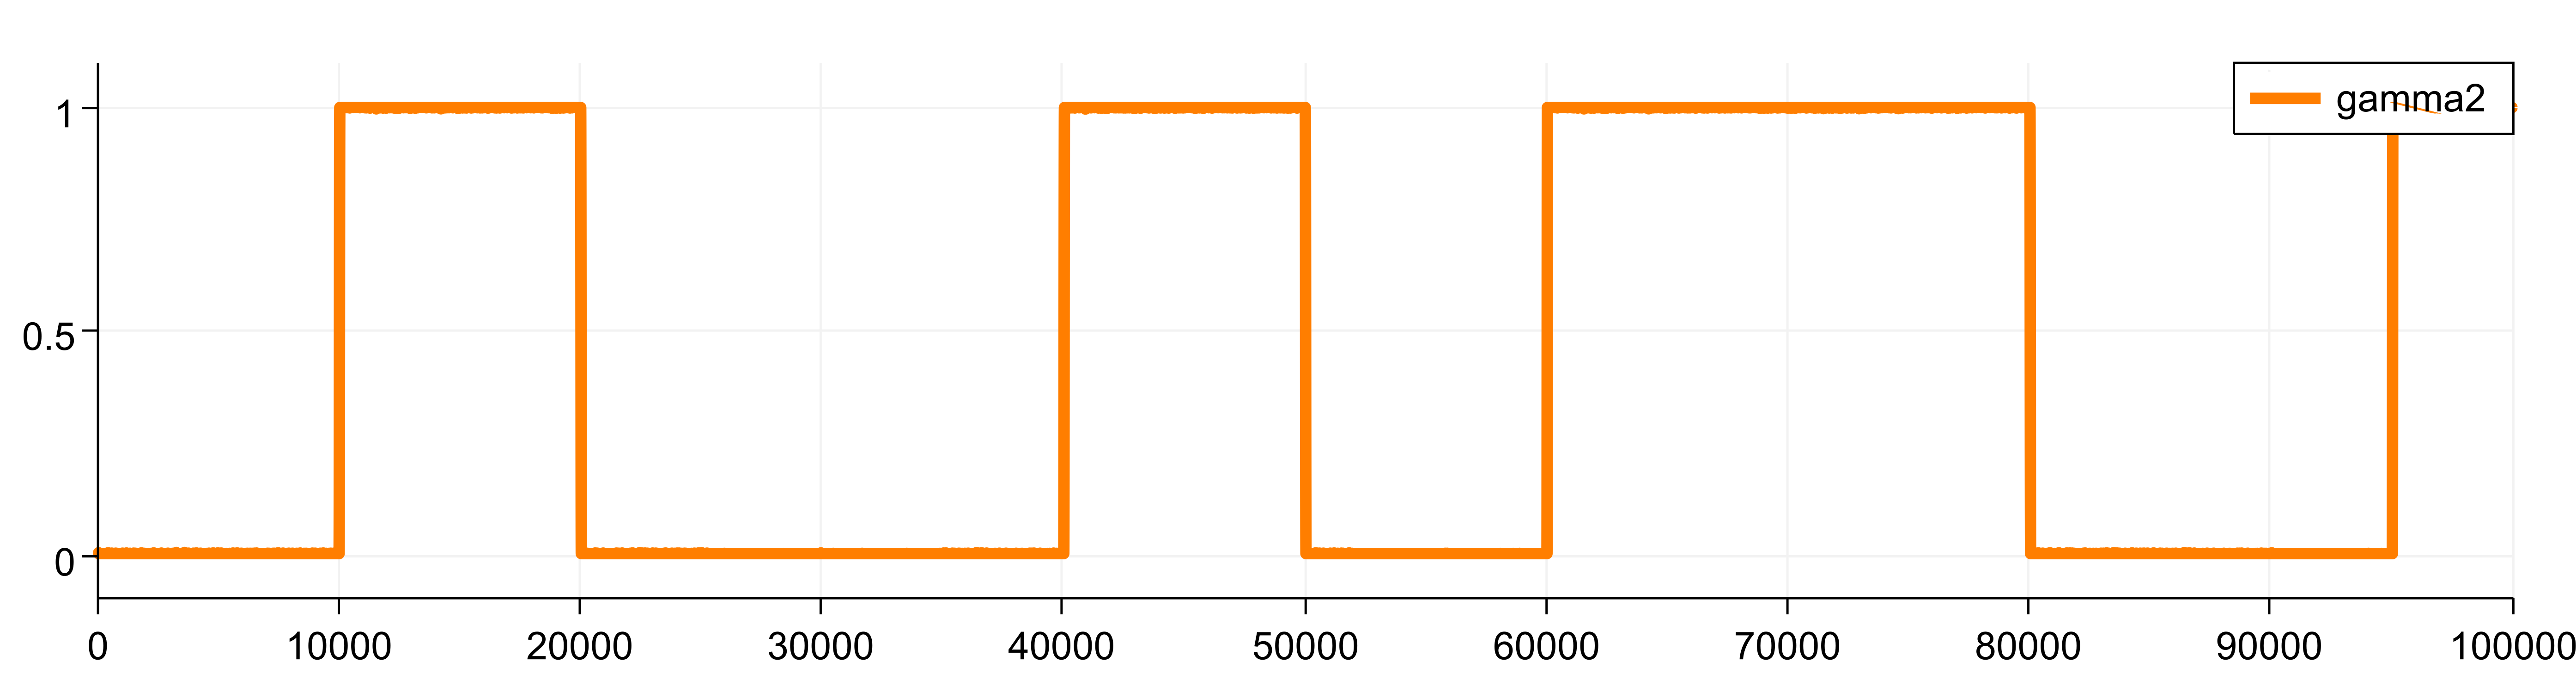
\includegraphics[width=1.0\linewidth, angle=0, clip = true]{figures/gamma2.png} 

			\caption{The solution - indicator model function in FEM-BV-H1 model found using our new library. 
					 Library generates files suitable for ParaView.
					 }
			\label{fig:indicator}	
		\end{center}
	\end{figure}
	\begin{figure}[H]
		\begin{center}
			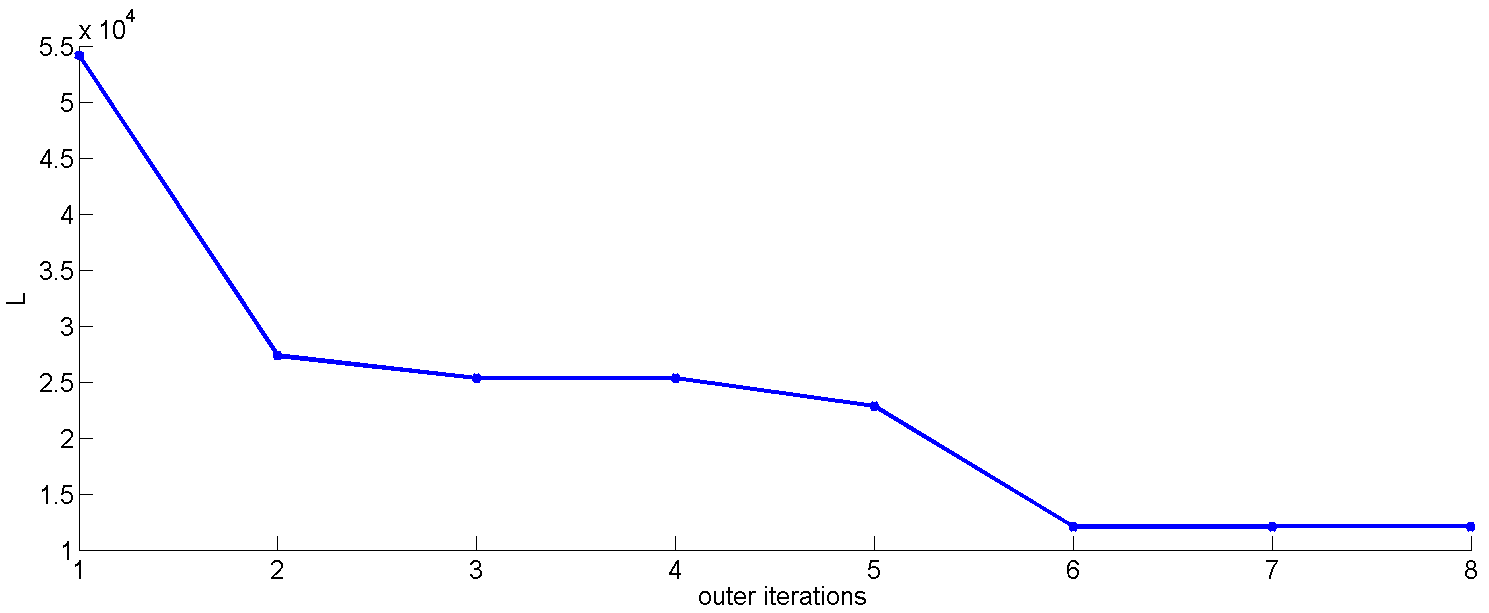
\includegraphics[width=1.0\linewidth, angle=0, clip = true]{figures/L.png} \\

			\caption{Monotone decrease of global objective function during outer iterations. Our algorithm is terminated when the difference of objective function is less than $10^{-4}$.
					 }
			\label{fig:L}	
		\end{center}
	\end{figure}
\end{column}	
\begin{column}{0.02\linewidth}\end{column}
\end{columns}





\end{block}



%----------------------------------------------------------------------------------------
%	REFERENCES
%----------------------------------------------------------------------------------------

\begin{block}{References}
        
\nocite{*} % Insert publications even if they are not cited in the poster
\small{

\bibliography{ams}
\bibliographystyle{apalike}
%\bibliographystyle{unsrt}

%% BIBLIOGRAPHY 
\begin{thebibliography}{}

\bibitem{brockwell2002}
P.~Brockwell and R.~Davis.
{\em Introduction to Time Series and Forecasting}.
Springer, Berlin, 2002.

\bibitem{granger69}
C.~Granger.
{\em Investigating causal relations by econometric models and cross-spectral methods}.
Econometrica, 37:424--438, 1969.

\bibitem{horenko_fem}
I.~Horenko.
{\em Finite Element Approach to Clustering of Multidimensional Time Series}.
SIAM J. Sci. Comp. 32, 62--83, 2010.

\bibitem{horenko_pnas_2014}
S.~Gerber and I.~Horenko.
{\em On inference of causality for discrete state models in a multiscale context}.
Proc. Natl. Acad. Sci. USA (PNAS), 2014.

\bibitem{metzner_2012}
P.~Metzner, L.~Putzig, and I.~Horenko.
{\em Analysis of persistent non-stationary time series and applications}.
 CAMCoS 7, 175--229, 2012.

\bibitem{pospisil_phd}
L.~Pospisil.
{\em Development of Algorithms for Solving Minimizing Problems
with Convex Quadratic Function on Special Convex Sets and Applications}.
PhD thesis, supervised by Z.~Dostal, VSB-TU Ostrava, 2014.

\bibitem{spg}
E.G.~Birgin, J.M~Martinez, and M.M.~Raydan.
{\em Nonmonotone spectral projected gradient methods on convex sets}. 
SIAM Journal on Optimization 10, 1196--1211, 2000.

\bibitem{simplex}
Y.~Chen, X.~Ye.
{\em Projection Onto A Simplex}.
Arxiv. 1101.6081, 2012.


\end{thebibliography}

}

\end{block}




%----------------------------------------------------------------------------------------

\end{column} % End of the second column

\begin{column}{.008\textwidth}\end{column} % Empty spacer column

\end{columns} % End of all the columns in the poster

\end{frame} % End of the enclosing frame

\end{document}
